\subsubsection{The problem of Pipeline Hazards}\label{subsubsection: The problem of Pipeline Hazards}

\begin{definitionbox}
    A \definition{hazard (conflict)} is created whenever there a \textbf{dependence} between two instructions, and instructions are close enough that the overlap caused by pipelining would change the order of access to the operands involved in the dependence.
\end{definitionbox}

\begin{flushleft}
    \textcolor{Red2}{\faIcon{exclamation-triangle} \textbf{Problem Consequences}}
\end{flushleft}
The Hazards:
\begin{itemize}
    \item \textbf{Force} the next \textbf{instruction} in the pipeline \textbf{to be executed later} than its intended clock cycle.

    \item \textbf{Reduced the performance} from the ideal speedup achieved by pipelining (direct previous consequence).
\end{itemize}
There are \textbf{three classes} of Hazards:
\begin{itemize}
    \item \definition{Structural Hazards}. Attempt to use the \textbf{same resource from different instructions simultaneously}.
    
    \example{Example}: single memory for instruction and data.
    

    \item \definition{Data Hazards}. Attempt to \textbf{use a result before it is ready}.
    
    \example{Example}: instruction depending on a result of a previous instruction still in the pipeline.

    There are also \textbf{two specific forms} of data hazard, called \definition{Load-Use Data Hazard} and \definition{Load-Store Data Hazard}. Both occur when the \textbf{data loaded by a load instruction is not yet available when it is needed by another instruction}. In the case of Load-Use, the \dquotes{another instruction} is an operator such as \texttt{add}; in the case of Load-Store, the \dquotes{another instruction} is the store (\texttt{sw}) instruction.

    The following \example{example} shows the conflict (Load-Use Data Hazard) between two instructions. In particular, the value \texttt{lw} writes to \texttt{s2} is not available until \texttt{lw} has completed the \texttt{MEM} phase, but \texttt{and} needs this value when it enters the \texttt{EX} phase, i.e. when \texttt{lw} enters the \texttt{MEM} phase.
    \lstinputlisting[language=misc]{code/the-problem-of-pipeline-hazards/load-use-data-hazard.s}

    \item \definition{Control Hazards}. Attempt to \textbf{make a decision on the next instruction to execute before the condition is evaluated}.
    
    \example{Example}: conditional branch execution.
\end{itemize}

\begin{flushleft}
    Structural Hazards? No problem for MIPS Architecture!
\end{flushleft}
\textbf{There aren't any structural hazards in MIPS architecture} because the Instruction Memory (IM) is separated from the Data Memory (DM). Also, the Register File (RF) is used in the same clock cycle (read access by an instruction and write access by another instruction).

\newpage

\begin{flushleft}
    \textcolor{Green3}{\faIcon{question-circle} \textbf{How to detect Data Hazards? Dependency Analysis}}
\end{flushleft}
To \textbf{detect Data Hazards}, it is suggested to analyze the dependencies. If the instructions executed in the pipeline depend on each other, data hazards can arise \textbf{when instructions are too close}. For \example{example}:
\lstinputlisting[language=misc]{code/the-problem-of-pipeline-hazards/data-hazards-1.s}
Data Hazards can occur in a variety of situations, but a \textbf{true dependency situation} is created by a \textbf{RAW (Read After Write) Hazard}.

\begin{definitionbox}
    A \definition{RAW (Read After Write) Hazard} occurs when an instruction $n+1$ tries to read a source operand before the previous instruction $n$ has written its value in the Register File (RF).
\end{definitionbox}

\noindent
For \example{example}:
\lstinputlisting[language=misc]{code/the-problem-of-pipeline-hazards/RAW-hazard-1.s}

\begin{center}
    \large
    \textcolor{Red3}{\textbf{MIPS Optimized Pipeline}}
\end{center}
Consider the following situation:
\begin{figure}[!htp]
    \centering
    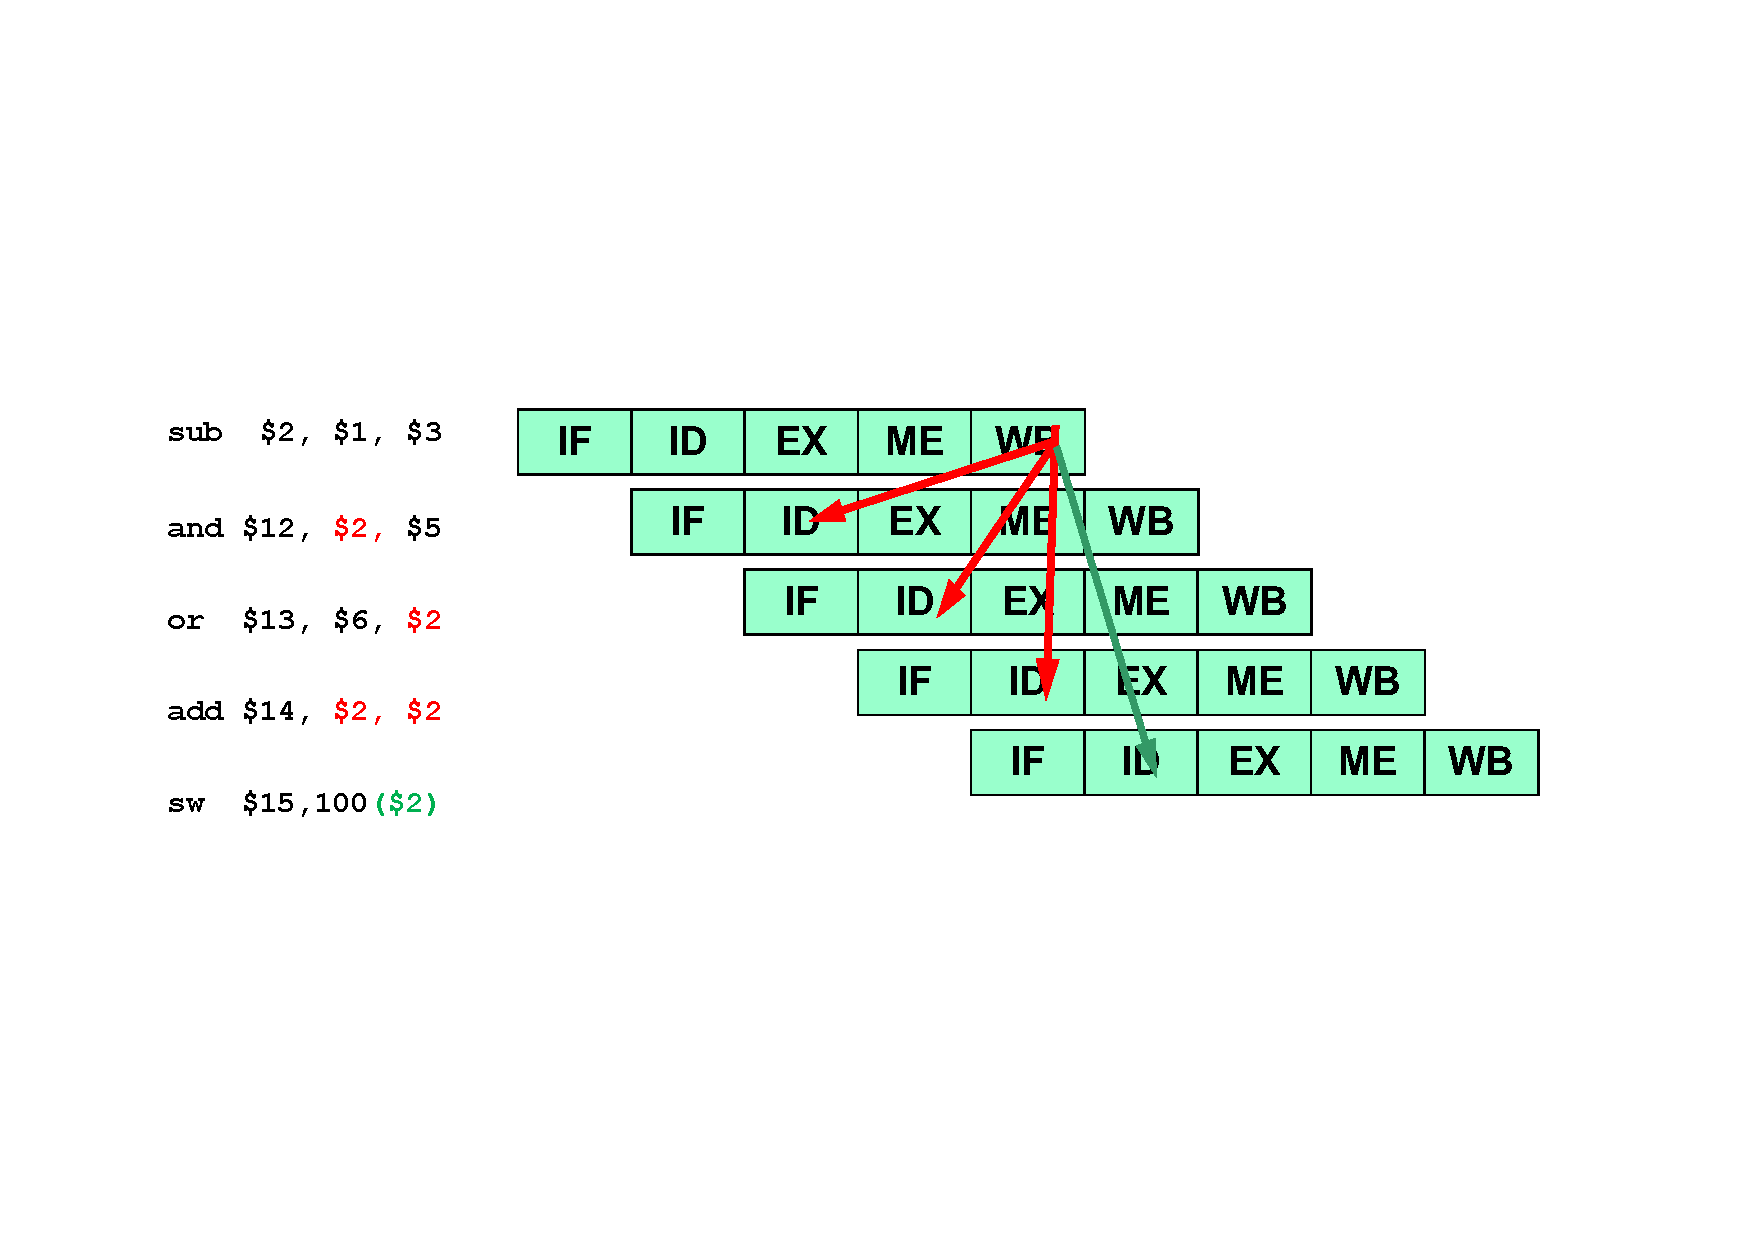
\includegraphics[width=\textwidth]{img/RAW-hazards-1.pdf}
    \caption{Why MIPS Optimized Pipeline was born.\cite{pipelining-slides}}
\end{figure}

\noindent
The Register File is used in 2 stages: read access during ID (\texttt{and} operation) and write access during Write Back (WB) (\texttt{sub} operation). \emph{What happens if read and write refer to the same register in the same clock cycle?} Or we insert a stall, or we use an \textbf{optimized pipeline} (smart choice).

\begin{definitionbox}
    By selecting \definition{Optimized Pipeline}, we assume the Register File (RF) read occurs in the second half of clock cycle and the Register File write in the first half of clock cycle.
\end{definitionbox}

\noindent
This way \textbf{we don't need the stall}. The following Figure~\ref{fig: Optimized Pipeline} shows an optimized pipeline.

\newpage

\begin{figure}[!htp]
    \centering
    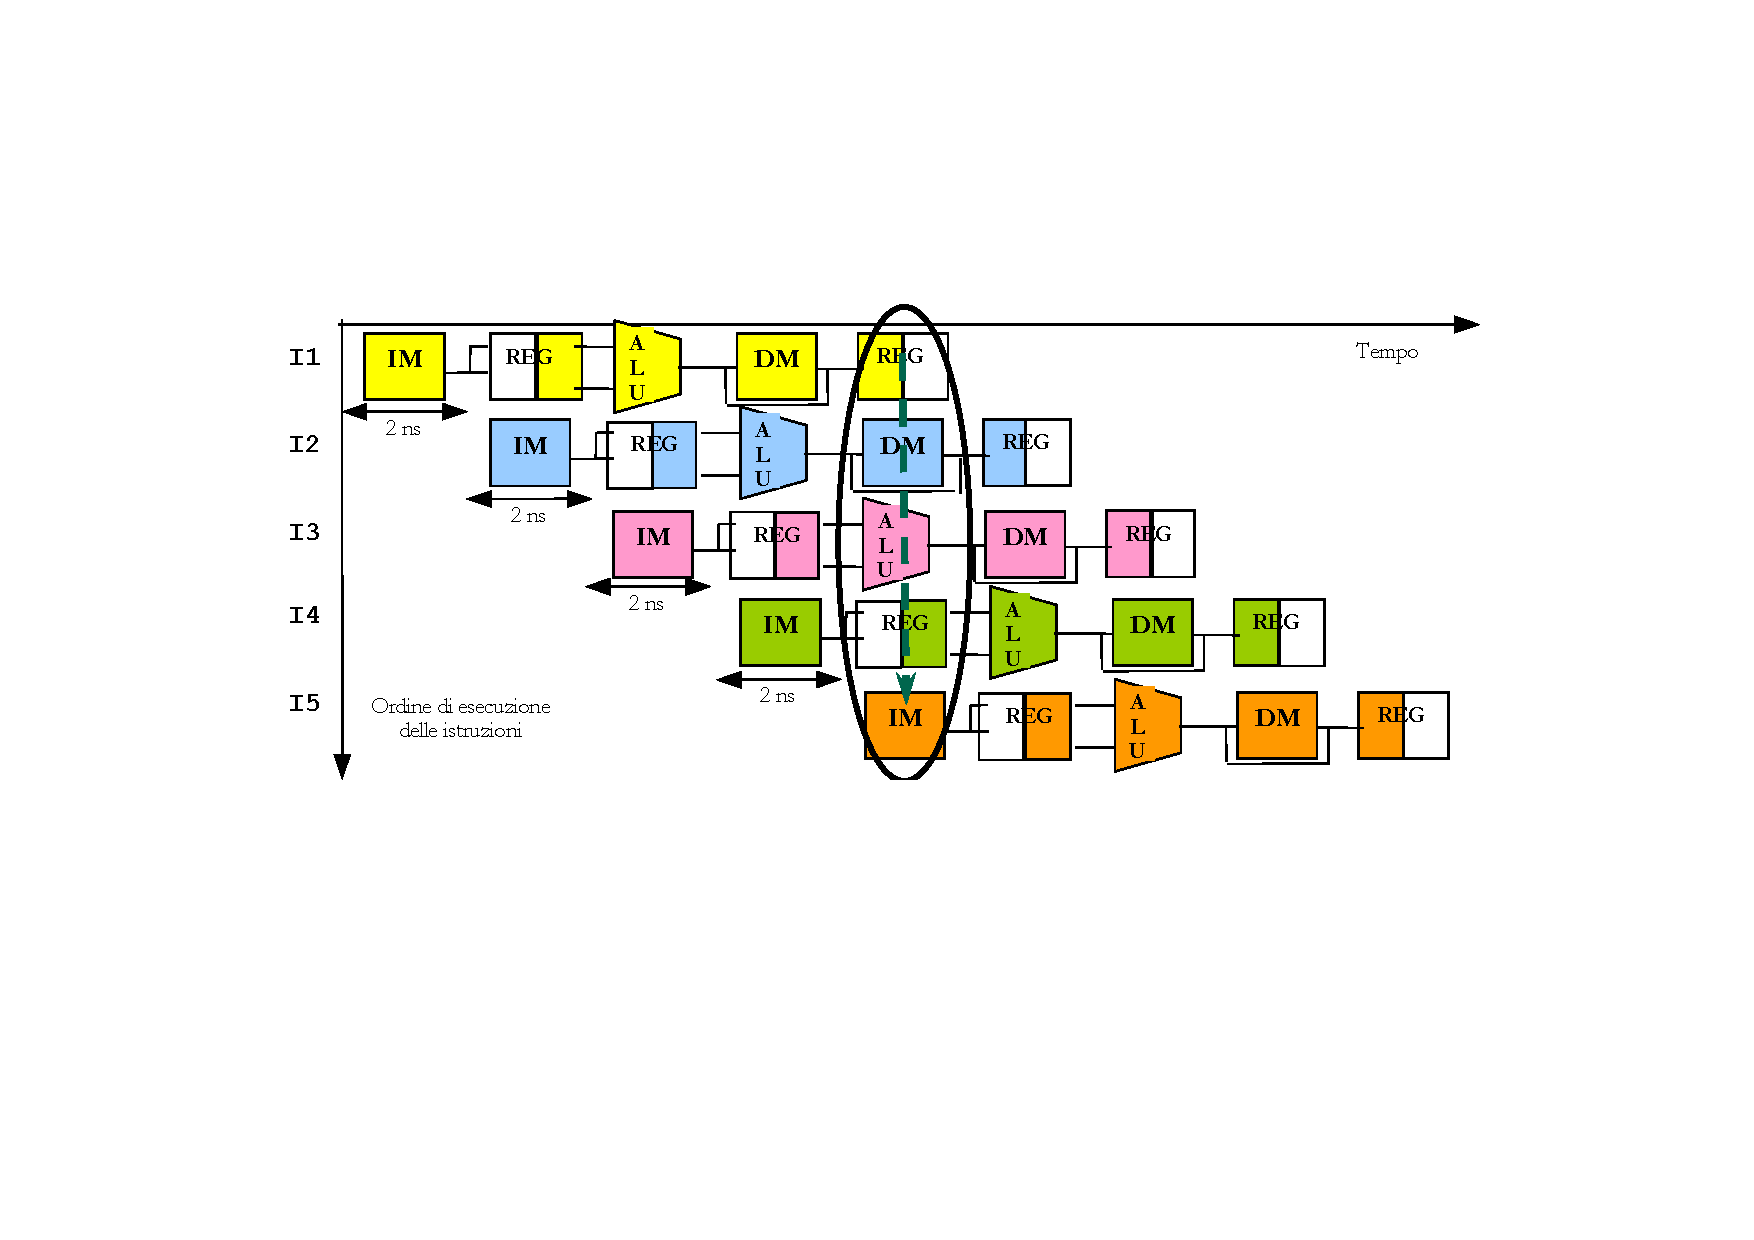
\includegraphics[width=\textwidth]{img/optimized-pipeline-1.pdf}
    \caption{Optimized Pipeline (IM is Instruction Memory, REG is Register File, and DM is Data Memory).\cite{pipelining-slides}}
    \label{fig: Optimized Pipeline}
\end{figure}

\noindent
And the problem mentioned at the beginning of this paragraph is partially solved, as we can see in the following figure.
\begin{figure}[!htp]
    \centering
    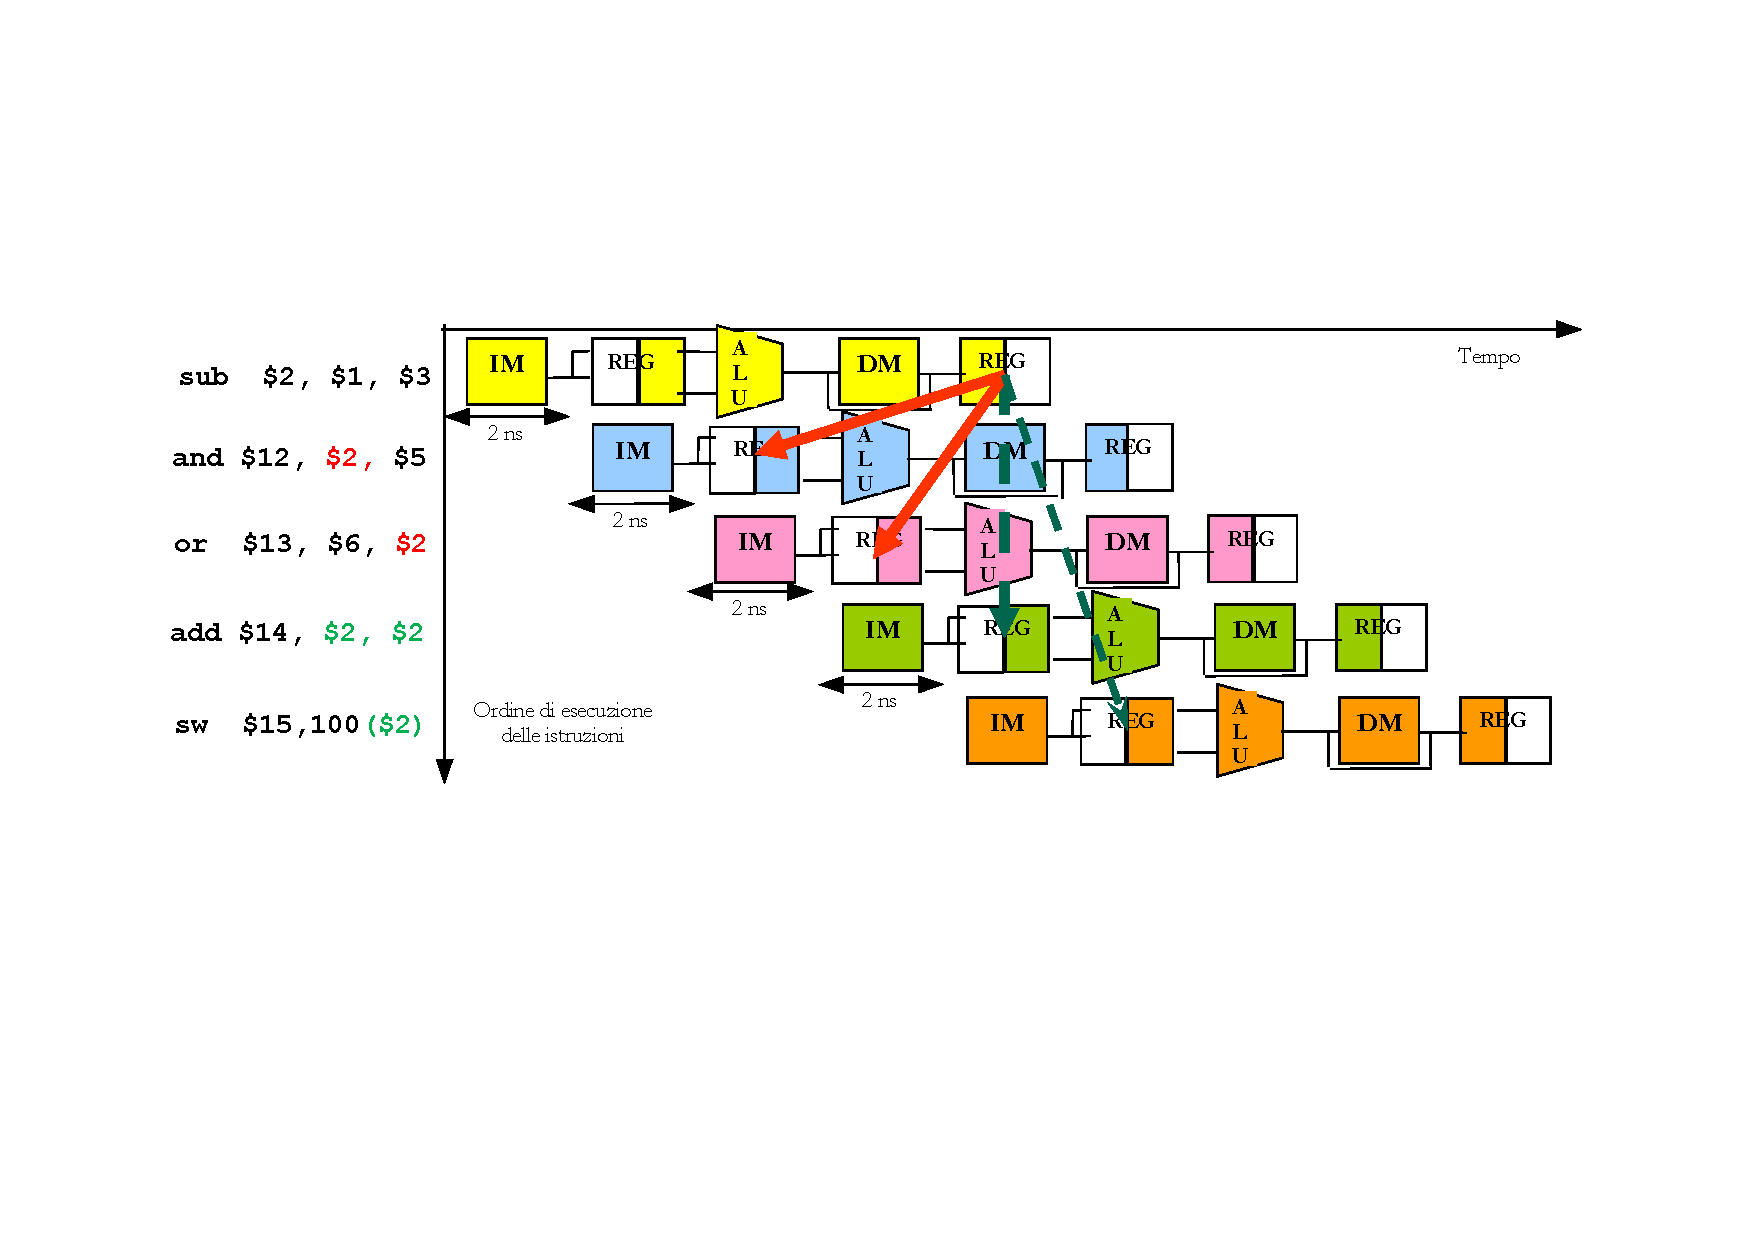
\includegraphics[width=\textwidth]{img/optimized-pipeline-2.pdf}
    \caption{Optimized Pipeline to solve the example stall.\cite{pipelining-slides}}
\end{figure}